\chapter{溶液与溶解度}\label{ch:g6:solutions-and-solubility}

打开一瓶气泡水时，先是“嘶”的一声，一簇细小的气泡
仿佛凭空冒出。一秒钟之前，水看上去还完全澄清，
其实气体早已溶解在其中。固体会溶解，液体会溶解，
气体也会溶解，但溶解从来不是没有限度的。
本章将说明溶液的各个组成部分，
并测定液体最多能溶解多少某种物质。

\begin{recall}
溶于水的固体会从视野中消失，液体保持澄清；这种澄清的液体即为溶液，
其中仍然含有所溶解的物质（\cref{ch:g2:mixing-and-dissolving}）。
溶液是化学物种的均相混合物
（\cref{ch:g6:pure-substances-and-mixtures}）。
蒸发掉水，
即可重新得到溶解的固体（\cref{ch:g3:separating-mixtures}）。
\end{recall}

\begin{omfigure}
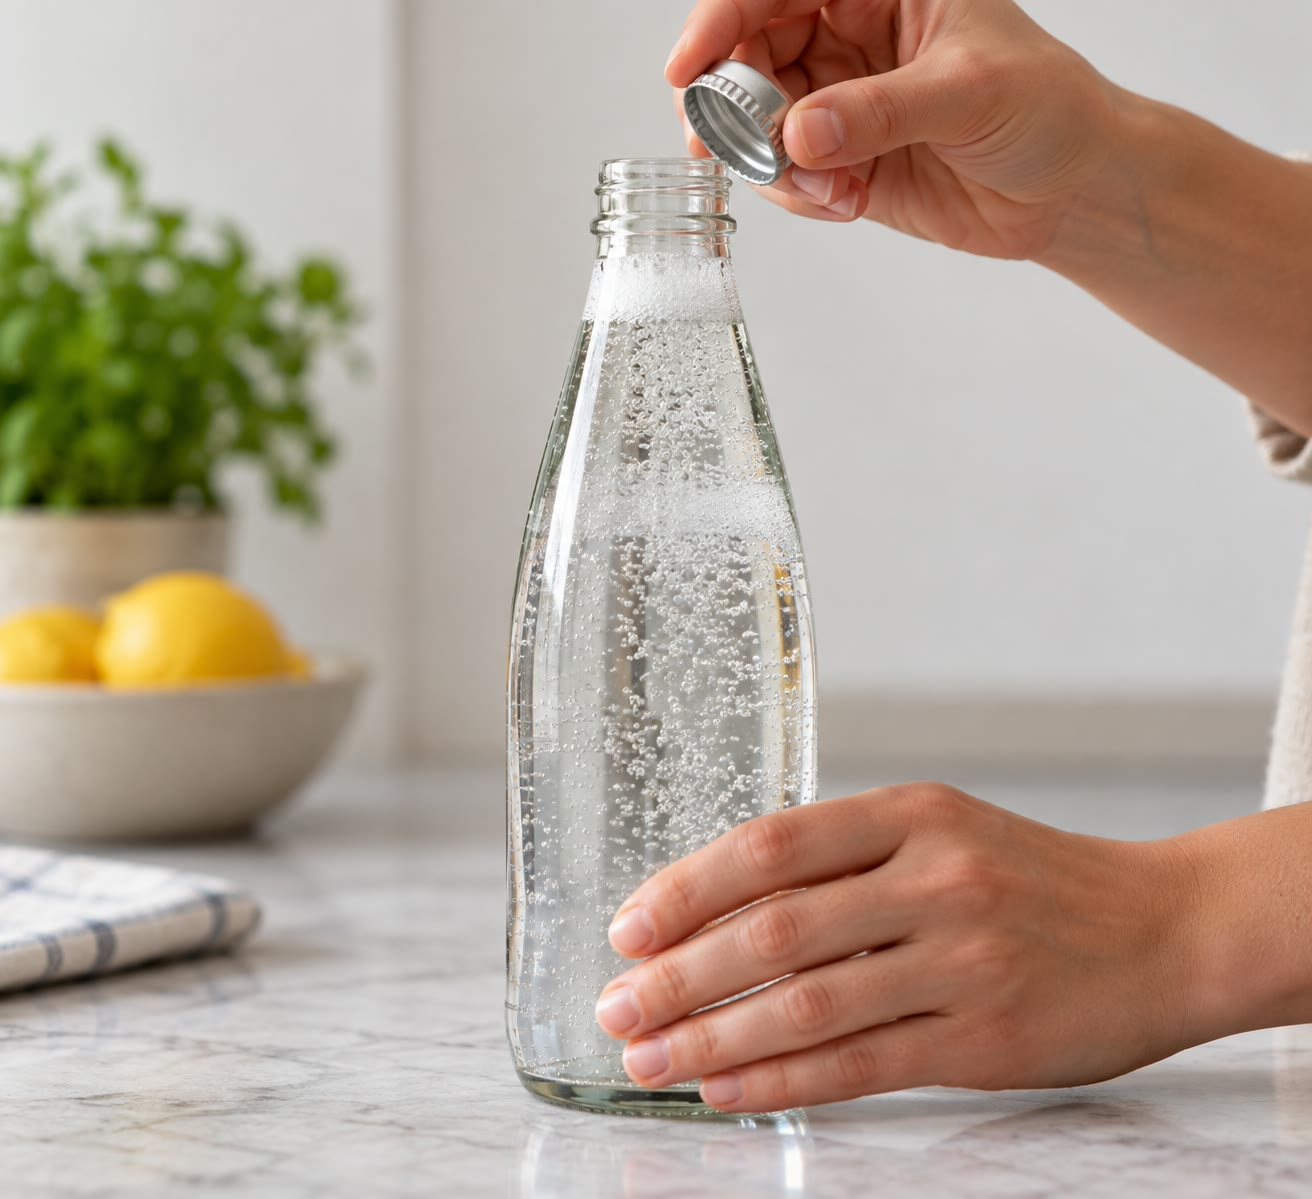
\includegraphics[width=0.5\linewidth]{images/book1/ai/g6-fizzy-water.jpg}

{\small 打开一瓶气泡水时：溶解的气体
以气泡的形式逸出。}
\end{omfigure}

\section{溶质与溶剂}

\begin{definition}[溶质、溶剂、水溶液]\label{def:g6:solutions-and-solubility:solute}
在溶液中，能够溶解的物质称为
\emph{溶质}\index{溶质}，能溶解溶质的液体称为
\emph{溶剂}\index{溶剂}。溶剂为水时，溶液
称为\emph{水溶液}\index{水溶液}。
\end{definition}

\begin{example}[除水以外的溶剂]\label{ex:g6:solutions-and-solubility:solvents}
水是最常见的溶剂，但并非唯一的溶剂。指甲油不溶于水，
而溶于丙酮，丙酮是指甲油去除剂中的溶剂。
油脂和油画颜料可溶于矿物松节油。
许多药物是溶于乙醇中的。一种溶液可以含有多种溶质：
海水中溶有食盐和许多其他物质。
\end{example}

\begin{safety}{\ghs{GHS02}\ghs{GHS07}}
% ledger: ghs:acetone
丙酮：高度易燃的液体和蒸气（GHS02）；它会刺激眼睛，
其蒸气可能使人昏昏欲睡或头晕（GHS07）。
使用时应在通风的房间内进行，远离一切明火。
\end{safety}

\begin{proposition}[质量相加]\label{prop:g6:solutions-and-solubility:mass}
溶液的质量等于溶剂的质量与
所溶解溶质的质量之和：固体溶解时并无质量损失，
尽管它已不可见。
\end{proposition}

\begin{omfigure}
\begin{tikzpicture}[font=\small, scale=1.15]
  \pic[transform shape] at (0,0) {balance};
  \pic[transform shape] at (0,0.8) {beaker={0.5}{omWater!80}};
  \node[anchor=north, align=center] at (0,-0.1) {\qty{100}{g}的水};
  \node at (1.85,1.3) {$+$};
  \pic[transform shape] at (3.5,0) {balance};
  \fill[white, draw=black!45] (3.0,0.8) rectangle (4.0,0.9);
  \fill[white, draw=black!45] (3.15,0.9) -- (3.85,0.9) -- (3.5,1.2) -- cycle;
  \node[anchor=north, align=center] at (3.5,-0.1) {\qty{10}{g}的糖};
  \draw[->, thick, omProp] (4.9,1.2) -- (6.0,1.2) node[midway, above, text=black]
    {搅拌};
  \pic[transform shape] at (7.4,0) {balance};
  \pic[transform shape] at (7.4,0.8) {beaker={0.52}{omWater!80}};
  \node[anchor=north, align=center] at (7.4,-0.1) {\qty{110}{g}的糖水};
\end{tikzpicture}

{\small 将\qty{10}{g}糖溶于\qty{100}{g}水中，得到
\qty{110}{g}溶液（忽略烧杯的质量）。}
\end{omfigure}

\section{饱和与溶解度}

\begin{definition}[饱和溶液]\label{def:g6:solutions-and-solubility:saturated}
若溶液已无法再溶解其溶质，则称为\emph{饱和溶液}\index{饱和溶液}：
此时加入的任何溶质都会留在底部，不再溶解，
无论搅拌多久。
\end{definition}

\begin{definition}[溶解度]\label{def:g6:solutions-and-solubility:solubility}
溶质在溶剂中的\emph{溶解度}\index{溶解度}，是指
在一定温度下，一定量的溶剂最多能溶解的溶质质量。
对于固体在水中的溶解度，常以
每升（或每千克）水中所能溶解的克数表示。
\end{definition}

\begin{proposition}[一些物质在水中的溶解度]\label{prop:g6:solutions-and-solubility:values}
% ledger: sol:NaCl, sol:sucrose, sol:CO2, sol:O2 (O2: 31 mL/L, 31/24.0 x 32 = 0.041 g/L at 20 C)
实测表明，各种物质在水中的溶解度差别极大：
\begin{center}
\small
\begin{tabular}{lll}
\hline
溶质 & 在水中的溶解度 & 条件 \\
\hline
蔗糖 & 每升水约 \qty{2000}{g} & 室温 \\
食盐（氯化钠） & 每千克水 \qty{360}{g} & \qty{25}{\celsius} \\
二氧化碳 & 每升约 \qty{1.5}{g} & \qty{25}{\celsius}，该气体压强下 \\
氧气 & 每升约 \qty{0.04}{g} & \qty{20}{\celsius}，该气体压强下 \\
沙子、白垩 & 几乎不溶 &——\\
\hline
\end{tabular}
\end{center}
一升水能溶解的蔗糖超过其自身的质量，
却连半克氧气都溶解不了。
\end{proposition}

\begin{method}[能否全部溶解？]\label{met:g6:solutions-and-solubility:will-it}
要判断质量为 $m$ 的溶质能否完全溶解于一定体积的
水中，可按以下步骤进行：
\begin{enumerate}
  \item 查出溶质的溶解度（单位：克每升水）；
  \item 计算该体积的水最多能溶解的质量；
  \item 比较 $m$ 与该质量：若 $m$ 较小，则全部溶解；若 $m$
        较大，则溶液已饱和，多余的部分
        留在底部。
\end{enumerate}
\end{method}

\begin{example}[杯中的食盐]\label{ex:g6:solutions-and-solubility:glass}
% ledger: sol:NaCl
能否将 \qty{50}{g} 食盐溶于 \qty{200}{mL} 水中（约
\qty{200}{g}）？一千克水最多溶解 \qty{360}{g} 食盐，
故 \qty{200}{g} 水最多可溶解 $360 \times
\frac{200}{1000} = \qty{72}{g}$。因 $50 < 72$，食盐
全部溶解。
\end{example}

\begin{omfigure}
\begin{tikzpicture}[font=\small, scale=1.15]
  \pic[transform shape] at (0,0) {beaker={0.6}{omWater!80}};
  \node[anchor=north, align=center] at (0,-0.15) {少量食盐：\\ 全部溶解};
  \pic[transform shape] at (3.2,0) {beaker={0.6}{omWater!80}};
  \node[anchor=north, align=center] at (3.2,-0.15) {较多食盐：\\ 恰好饱和};
  \pic[transform shape] at (6.4,0) {beaker={0.6}{omWater!80}};
  \fill[black!12, draw=black!50] (5.7,0) -- (7.1,0) -- (6.9,0.2) -- (5.9,0.2) -- cycle;
  \foreach \x in {5.85,6.05,6.25,6.45,6.65,6.85} \fill[black!45] (\x,0.09) circle (0.03);
  \node[anchor=north, align=center] at (6.4,-0.15) {食盐过多：\\ 剩余部分不溶解};
\end{tikzpicture}

{\small 向同一杯水中不断加入食盐。溶液一旦
饱和，多余的食盐便留在底部。}
\end{omfigure}

\begin{inthelab}[盐水的饱和]
老师每次向 \qty{100}{mL} 水中加入一勺食盐，
每次加入后充分搅拌。开始的几勺都溶解了；随后加入的一勺
不能再完全溶解，白色颗粒留在
底部：溶液已饱和。称得所用食盐的质量表明
约有 \qty{36}{g} 食盐溶解了。
\end{inthelab}

\section{互溶与不互溶的液体}

\begin{definition}[互溶与不互溶的液体]\label{def:g6:solutions-and-solubility:miscible}
两种液体混合在一起，若得到单一的均匀液体，则称二者为\emph{互溶的}\index{互溶的}；
若混合后分为两层，则称二者为
\emph{不互溶的}\index{不互溶的}，
较轻的一层在上。
\end{definition}

\begin{example}[水与乙醇、水与油]\label{ex:g6:solutions-and-solubility:liquids}
水与乙醇互溶：振荡混合后，得到一种澄清的
液体。水与油不互溶：无论怎样用力振荡，
油会重新浮起，在水面上形成独立的一层。在一罐沙拉酱中，
油漂浮在醋的上方，醋主要
是水。
\end{example}

\begin{omfigure}
\begin{tikzpicture}[font=\small, scale=1.3]
  \pic[transform shape] at (0,0) {testtube={0.6}{omWater!80}};
  \node[anchor=north, align=center] at (0,-0.15) {水 + 乙醇：\\ 一层};
  \pic[transform shape] at (3,0) {testtube={0.65}{yellow!55!orange!60}};
  \begin{scope}
    \clip (2.75,3) -- (2.75,0.25) arc[start angle=180, end angle=360, radius=0.25]
      -- (3.25,3) -- cycle;
    \fill[omWater!80] (2.7,0) rectangle (3.3,1.1);
  \end{scope}
  \draw[omGlass, line width=0.7pt] (2.75,3) -- (2.75,0.25) arc[start angle=180,
    end angle=360, radius=0.25] -- (3.25,3);
  \draw[<-, omProp, thick] (3.3,1.55) -- (4.1,1.75) node[right, text=black] {油};
  \draw[<-, omProp, thick] (3.3,0.6) -- (4.1,0.6) node[right, text=black] {水};
  \node[anchor=north, align=center] at (3,-0.15) {水 + 油：\\ 两层};
\end{tikzpicture}

{\small 互溶的液体只形成一层；不互溶的液体形成两层。}
\end{omfigure}

\begin{omfigure}
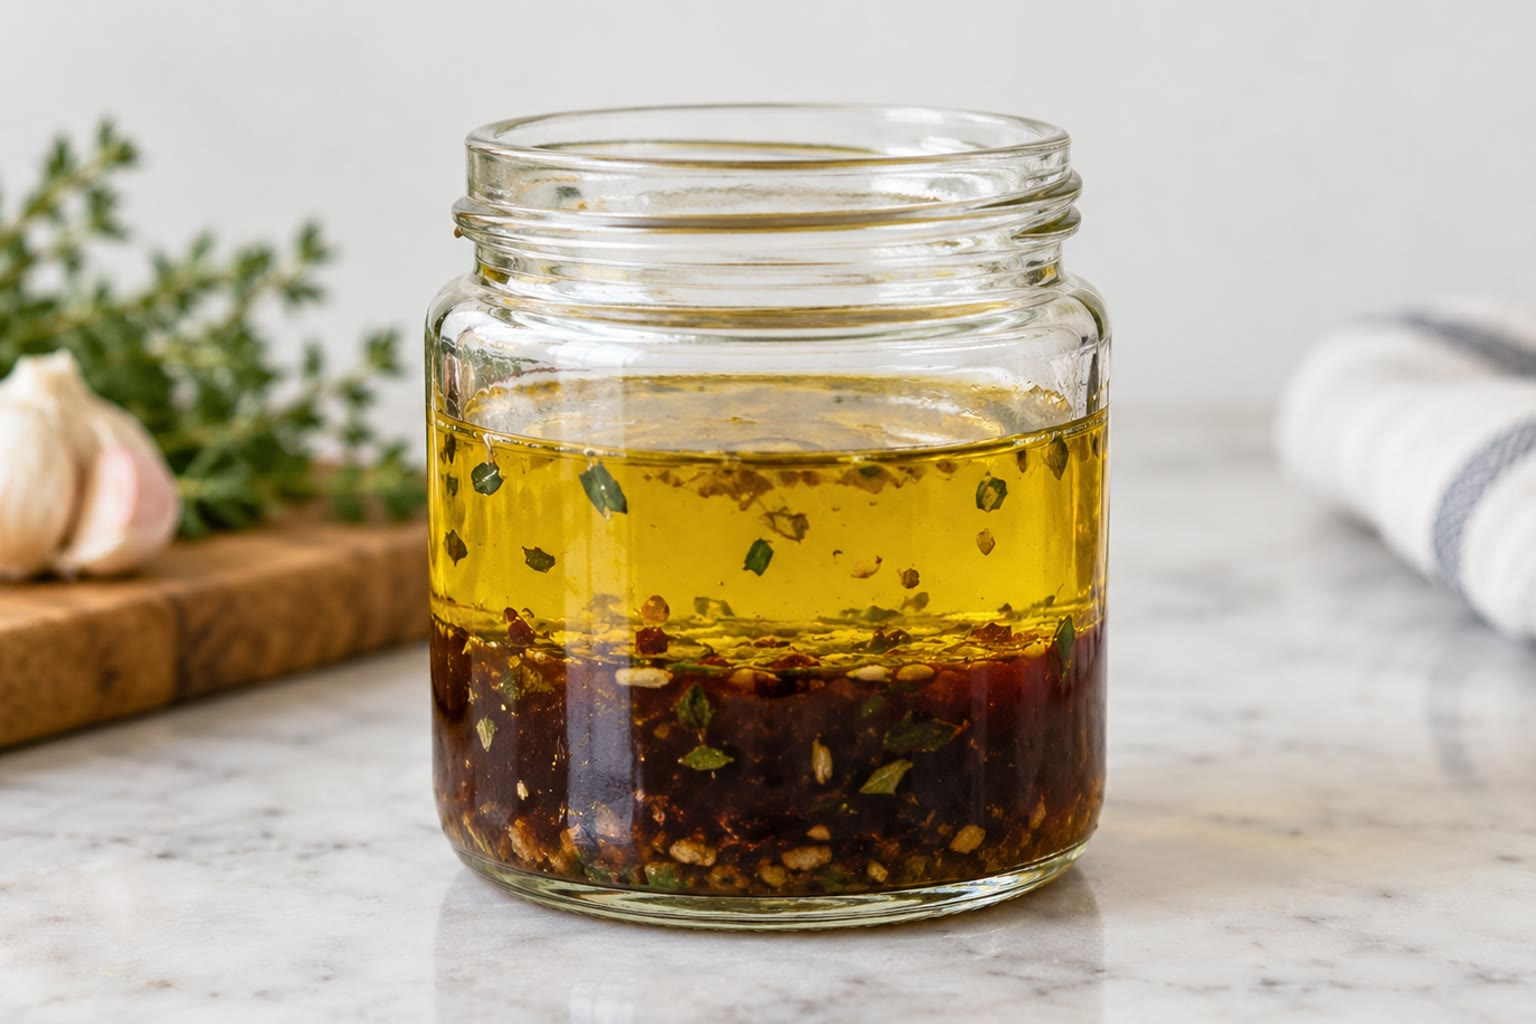
\includegraphics[width=0.45\linewidth]{images/book1/ai/g6-vinaigrette.jpg}

{\small 沙拉酱：油与醋不互溶。}
\end{omfigure}

\section{气体也能溶解}

\begin{proposition}[溶解的气体]\label{prop:g6:solutions-and-solubility:gases}
气体能溶于水，但量很少。汽水是
在密闭瓶中加压使二氧化碳溶入其中制成的；
打开瓶盖时，部分气体会以气泡的形式逸出。
与空气接触的水中溶有一定量的氧气，鱼类通过
鳃从水中获取氧气。气体在温水中的溶解量，比在冷水中
要少：温热的汽水会更快失去气泡。
\end{proposition}

\begin{example}[海洋与二氧化碳]\label{ex:g6:solutions-and-solubility:oceans}
海洋与空气接触的面积，约占地球表面的
三分之二。空气中的二氧化碳溶入海水，因此海洋
吸收了人类排放到空气中的部分二氧化碳。
\end{example}

\begin{omfigure}
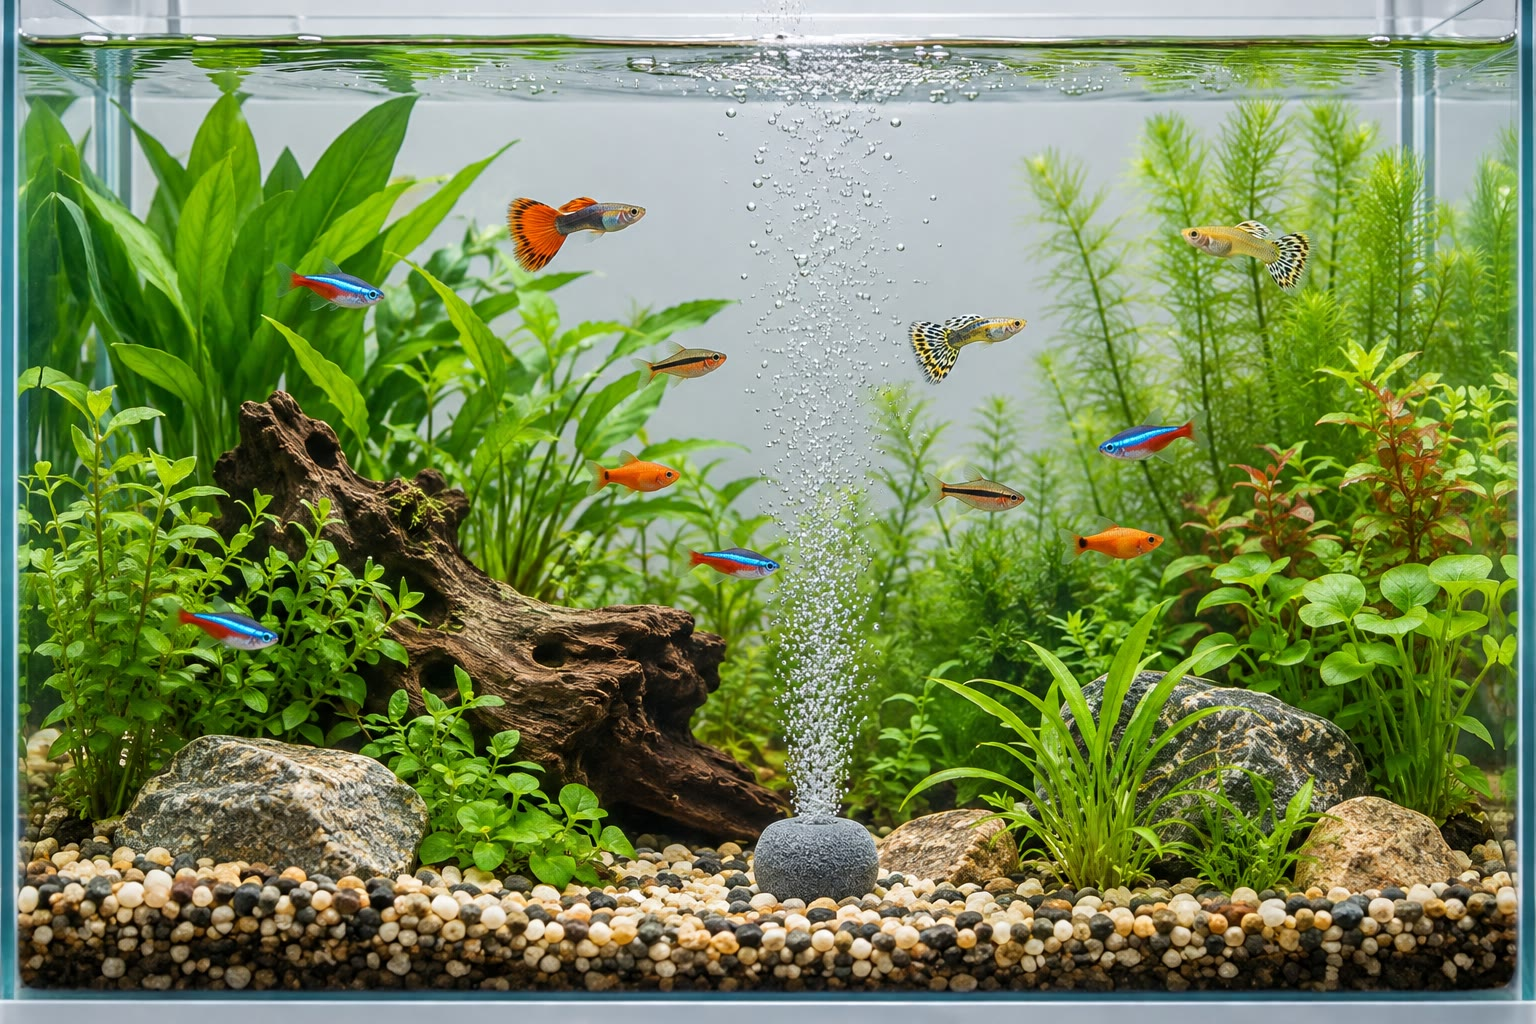
\includegraphics[width=0.5\linewidth]{images/book1/ai/g6-fish-tank.jpg}

{\small 鱼缸：气泡使水中不断补充
供鱼呼吸的溶解氧。}
\end{omfigure}

\section{练习}

\begin{exercise}[$\star$]\label{exo:g6:solutions-and-solubility:1}
在糖水中，指出溶质和溶剂。它是
水溶液吗？
\end{exercise}

\begin{exercise}[$\star$]\label{exo:g6:solutions-and-solubility:2}
什么是饱和溶液？怎样看出一种溶液
是饱和的？
\end{exercise}

\begin{exercise}[$\star$]\label{exo:g6:solutions-and-solubility:3}
将 \qty{20}{g} 食盐溶于 \qty{250}{g} 水中。溶液的
质量是多少？
\end{exercise}

\begin{exercise}[$\star$]\label{exo:g6:solutions-and-solubility:4}
判断下列物质与水是互溶的还是不互溶的：乙醇、食用油、食醋？
\end{exercise}

\begin{exercise}[$\star$]\label{exo:g6:solutions-and-solubility:5}
指出指甲油去除剂的溶剂，并说明其
两个象形图的含义。
\end{exercise}

\begin{exercise}[$\star\star$]\label{exo:g6:solutions-and-solubility:6}
利用食盐的溶解度，求
\qty{500}{g} 水在 \qty{25}{\celsius} 时最多能溶解的食盐质量。
\end{exercise}

\begin{exercise}[$\star\star$]\label{exo:g6:solutions-and-solubility:7}
将 \qty{80}{g} 食盐搅入 \qty{200}{g} 水中，
温度为 \qty{25}{\celsius}。能否全部溶解？若不能，
则底部剩余的质量是多少？
\end{exercise}

\begin{exercise}[$\star\star$]\label{exo:g6:solutions-and-solubility:8}
将 \qty{25}{g} 糖溶于 \qty{225}{g} 水中。糖
占溶液质量的百分之几？
\end{exercise}

\begin{exercise}[$\star\star$]\label{exo:g6:solutions-and-solubility:9}
观察三个盛有食盐水的烧杯的图，
哪个烧杯中还能继续溶解更多的食盐？
\end{exercise}

\begin{exercise}[$\star\star$]\label{exo:g6:solutions-and-solubility:10}
为什么汽水瓶打开时会冒出气泡，
而打开前却不会？
\end{exercise}

\begin{exercise}[$\star\star\star$]\label{exo:g6:solutions-and-solubility:11}
一升水大约能溶解 \qty{2000}{g} 糖，但
只能溶解约 \qty{0.04}{g} 氧气。糖的质量是氧气的
多少倍？
\end{exercise}

\begin{exercise}[$\star\star\star$]\label{exo:g6:solutions-and-solubility:12}
夏天，池塘水温升高，鱼会浮到水面
吸入空气。利用本章内容解释其原因。
\end{exercise}

\section{问题：奶酪师傅的盐水}

\begin{problem}[{周末问题——用于奶酪的饱和盐水
浴，以及夏季高温对它的影响}]
\label{pb:g6:solutions-and-solubility:1}
% ledger: sol:NaCl (360 g per kg of water; 1 L of water taken as 1 kg)
许多奶酪要在盐水浴中浸泡几小时。盐水是
食盐饱和的水。奶酪师傅向水箱中注入 \qty{20}{L} 的
水（\qty{20}{kg}），并加入食盐，直至底部
仍有少量食盐未溶解。取食盐的溶解度为每千克水
\qty{360}{g}。

\medskip
\noindent\textbf{第一部分——概念。}
\begin{enumerate}
  \item 在盐水中，哪一个是溶质，哪一个是溶剂？
  \item 对盐水而言，“饱和”是什么意思？
  \item 奶酪师傅为什么要不断加盐，直到
        底部留有少量食盐？
\end{enumerate}

\medskip
\noindent\textbf{第二部分——配制盐水。}
\begin{enumerate}[resume]
  \item \qty{20}{kg} 水中能溶解多少质量的食盐？
  \item 盐水的质量是多少（不计未溶解的食盐）？
  \item 食盐占盐水质量的百分之几？四舍五入
        四舍五入，取整数。
  \item 某天只加入 \qty{5}{kg} 食盐。盐水
        是否饱和？还能再溶解多少食盐？
\end{enumerate}

\medskip
\noindent\textbf{第三部分——炎热的夏天。}
炎热的一周里，\qty{5}{L}（\qty{5}{kg}）水从
第二部分的饱和盐水中蒸发，食盐没有损失。
\begin{enumerate}[resume]
  \item 水箱中还剩多少水？
  \item 这些水还能溶解多少质量的食盐？
  \item 剩余的水溶解不了的食盐会怎样？
  \item 奶酪师傅怎样凭肉眼就能看出
        这种情况已经出现？
  \item 计算水箱底部已结晶析出的
        食盐的质量。
\end{enumerate}
\end{problem}
